\documentclass[1p]{elsarticle_modified}
%\bibliographystyle{elsarticle-num}

%\usepackage[colorlinks]{hyperref}
%\usepackage{abbrmath_seonhwa} %\Abb, \Ascr, \Acal ,\Abf, \Afrak
\usepackage{amsfonts}
\usepackage{amssymb}
\usepackage{amsmath}
\usepackage{amsthm}
\usepackage{scalefnt}
\usepackage{amsbsy}
\usepackage{kotex}
\usepackage{caption}
\usepackage{subfig}
\usepackage{color}
\usepackage{graphicx}
\usepackage{xcolor} %% white, black, red, green, blue, cyan, magenta, yellow
\usepackage{float}
\usepackage{setspace}
\usepackage{hyperref}

\usepackage{tikz}
\usetikzlibrary{arrows}

\usepackage{multirow}
\usepackage{array} % fixed length table
\usepackage{hhline}

%%%%%%%%%%%%%%%%%%%%%
\makeatletter
\renewcommand*\env@matrix[1][\arraystretch]{%
	\edef\arraystretch{#1}%
	\hskip -\arraycolsep
	\let\@ifnextchar\new@ifnextchar
	\array{*\c@MaxMatrixCols c}}
\makeatother %https://tex.stackexchange.com/questions/14071/how-can-i-increase-the-line-spacing-in-a-matrix
%%%%%%%%%%%%%%%

\usepackage[normalem]{ulem}

\newcommand{\msout}[1]{\ifmmode\text{\sout{\ensuremath{#1}}}\else\sout{#1}\fi}
%SOURCE: \msout is \stkout macro in https://tex.stackexchange.com/questions/20609/strikeout-in-math-mode

\newcommand{\cancel}[1]{
	\ifmmode
	{\color{red}\msout{#1}}
	\else
	{\color{red}\sout{#1}}
	\fi
}

\newcommand{\add}[1]{
	{\color{blue}\uwave{#1}}
}

\newcommand{\replace}[2]{
	\ifmmode
	{\color{red}\msout{#1}}{\color{blue}\uwave{#2}}
	\else
	{\color{red}\sout{#1}}{\color{blue}\uwave{#2}}
	\fi
}

\newcommand{\Sol}{\mathcal{S}} %segment
\newcommand{\D}{D} %diagram
\newcommand{\A}{\mathcal{A}} %arc


%%%%%%%%%%%%%%%%%%%%%%%%%%%%%5 test

\def\sl{\operatorname{\textup{SL}}(2,\Cbb)}
\def\psl{\operatorname{\textup{PSL}}(2,\Cbb)}
\def\quan{\mkern 1mu \triangleright \mkern 1mu}

\theoremstyle{definition}
\newtheorem{thm}{Theorem}[section]
\newtheorem{prop}[thm]{Proposition}
\newtheorem{lem}[thm]{Lemma}
\newtheorem{ques}[thm]{Question}
\newtheorem{cor}[thm]{Corollary}
\newtheorem{defn}[thm]{Definition}
\newtheorem{exam}[thm]{Example}
\newtheorem{rmk}[thm]{Remark}
\newtheorem{alg}[thm]{Algorithm}

\newcommand{\I}{\sqrt{-1}}
\begin{document}

%\begin{frontmatter}
%
%\title{Boundary parabolic representations of knots up to 8 crossings}
%
%%% Group authors per affiliation:
%\author{Yunhi Cho} 
%\address{Department of Mathematics, University of Seoul, Seoul, Korea}
%\ead{yhcho@uos.ac.kr}
%
%
%\author{Seonhwa Kim} %\fnref{s_kim}}
%\address{Center for Geometry and Physics, Institute for Basic Science, Pohang, 37673, Korea}
%\ead{ryeona17@ibs.re.kr}
%
%\author{Hyuk Kim}
%\address{Department of Mathematical Sciences, Seoul National University, Seoul 08826, Korea}
%\ead{hyukkim@snu.ac.kr}
%
%\author{Seokbeom Yoon}
%\address{Department of Mathematical Sciences, Seoul National University, Seoul, 08826,  Korea}
%\ead{sbyoon15@snu.ac.kr}
%
%\begin{abstract}
%We find all boundary parabolic representation of knots up to 8 crossings.
%
%\end{abstract}
%\begin{keyword}
%    \MSC[2010] 57M25 
%\end{keyword}
%
%\end{frontmatter}

%\linenumbers
%\tableofcontents
%
\newcommand\colored[1]{\textcolor{white}{\rule[-0.35ex]{0.8em}{1.4ex}}\kern-0.8em\color{red} #1}%
%\newcommand\colored[1]{\textcolor{white}{ #1}\kern-2.17ex	\textcolor{white}{ #1}\kern-1.81ex	\textcolor{white}{ #1}\kern-2.15ex\color{red}#1	}

{\Large $\underline{12n_{0511}~(K12n_{0511})}$}

\setlength{\tabcolsep}{10pt}
\renewcommand{\arraystretch}{1.6}
\vspace{1cm}\begin{tabular}{m{100pt}>{\centering\arraybackslash}m{274pt}}
\multirow{5}{120pt}{
	\centering
	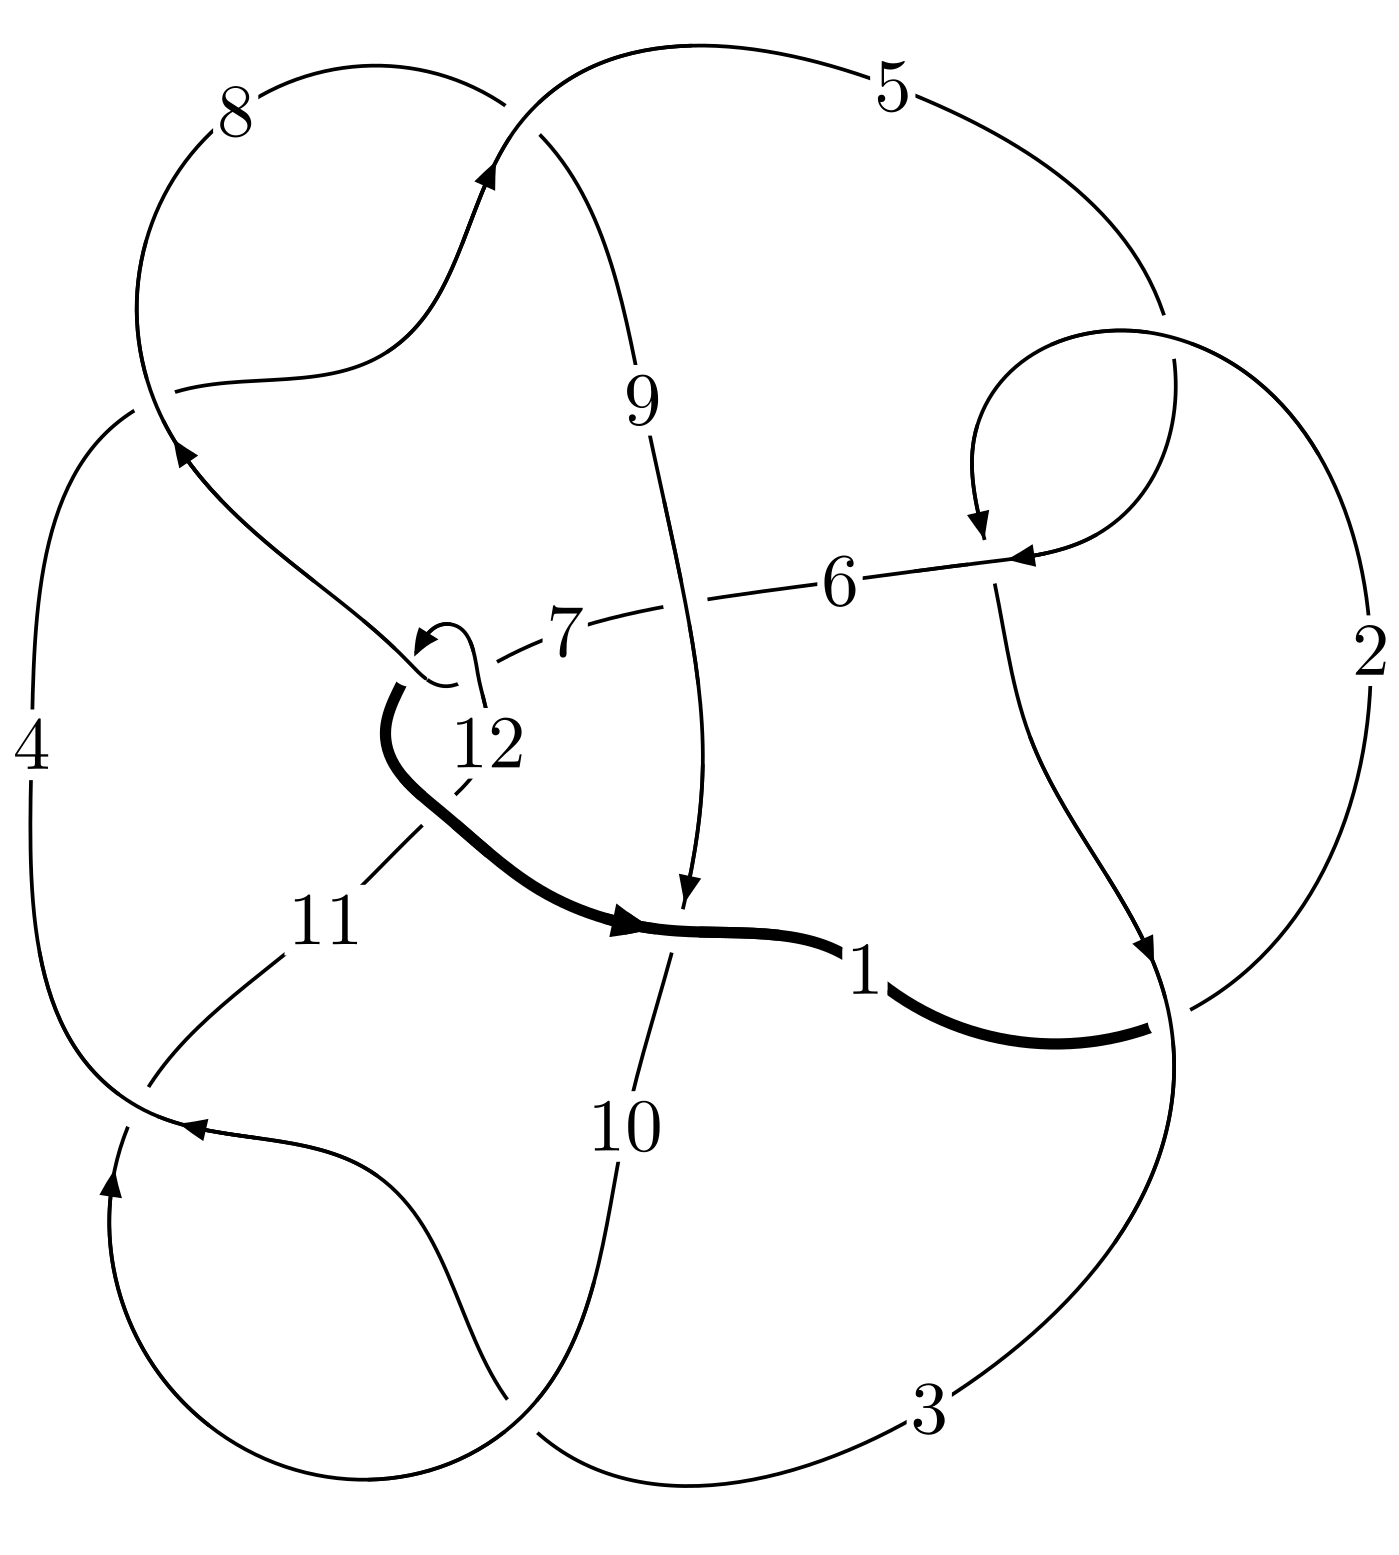
\includegraphics[width=112pt]{../../../GIT/diagram.site/Diagrams/png/2600_12n_0511.png}\\
\ \ \ A knot diagram\footnotemark}&
\allowdisplaybreaks
\textbf{Linearized knot diagam} \\
\cline{2-2}
 &
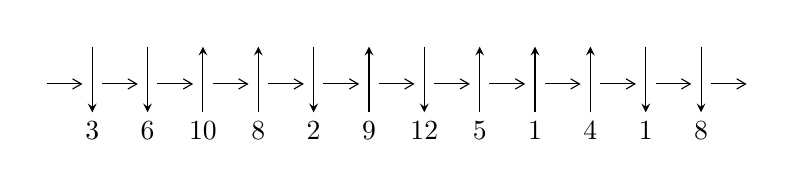
\begin{tikzpicture}[x=20pt, y=17pt]
	% nodes
	\node (C0) at (0, 0) {};
	\node (C1) at (1, 0) {};
	\node (C1U) at (1, +1) {};
	\node (C1D) at (1, -1) {3};

	\node (C2) at (2, 0) {};
	\node (C2U) at (2, +1) {};
	\node (C2D) at (2, -1) {6};

	\node (C3) at (3, 0) {};
	\node (C3U) at (3, +1) {};
	\node (C3D) at (3, -1) {10};

	\node (C4) at (4, 0) {};
	\node (C4U) at (4, +1) {};
	\node (C4D) at (4, -1) {8};

	\node (C5) at (5, 0) {};
	\node (C5U) at (5, +1) {};
	\node (C5D) at (5, -1) {2};

	\node (C6) at (6, 0) {};
	\node (C6U) at (6, +1) {};
	\node (C6D) at (6, -1) {9};

	\node (C7) at (7, 0) {};
	\node (C7U) at (7, +1) {};
	\node (C7D) at (7, -1) {12};

	\node (C8) at (8, 0) {};
	\node (C8U) at (8, +1) {};
	\node (C8D) at (8, -1) {5};

	\node (C9) at (9, 0) {};
	\node (C9U) at (9, +1) {};
	\node (C9D) at (9, -1) {1};

	\node (C10) at (10, 0) {};
	\node (C10U) at (10, +1) {};
	\node (C10D) at (10, -1) {4};

	\node (C11) at (11, 0) {};
	\node (C11U) at (11, +1) {};
	\node (C11D) at (11, -1) {1};

	\node (C12) at (12, 0) {};
	\node (C12U) at (12, +1) {};
	\node (C12D) at (12, -1) {8};
	\node (C13) at (13, 0) {};

	% arrows
	\draw[->,>={angle 60}]
	(C0) edge (C1) (C1) edge (C2) (C2) edge (C3) (C3) edge (C4) (C4) edge (C5) (C5) edge (C6) (C6) edge (C7) (C7) edge (C8) (C8) edge (C9) (C9) edge (C10) (C10) edge (C11) (C11) edge (C12) (C12) edge (C13) ;	\draw[->,>=stealth]
	(C1U) edge (C1D) (C2U) edge (C2D) (C3D) edge (C3U) (C4D) edge (C4U) (C5U) edge (C5D) (C6D) edge (C6U) (C7U) edge (C7D) (C8D) edge (C8U) (C9D) edge (C9U) (C10D) edge (C10U) (C11U) edge (C11D) (C12U) edge (C12D) ;
	\end{tikzpicture} \\
\hhline{~~} \\& 
\textbf{Solving Sequence} \\ \cline{2-2} 
 &
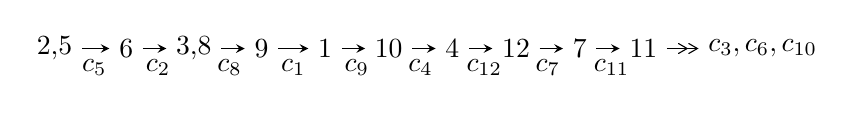
\begin{tikzpicture}[x=23pt, y=7pt]
	% node
	\node (A0) at (-1/8, 0) {2,5};
	\node (A1) at (1, 0) {6};
	\node (A2) at (33/16, 0) {3,8};
	\node (A3) at (25/8, 0) {9};
	\node (A4) at (33/8, 0) {1};
	\node (A5) at (41/8, 0) {10};
	\node (A6) at (49/8, 0) {4};
	\node (A7) at (57/8, 0) {12};
	\node (A8) at (65/8, 0) {7};
	\node (A9) at (73/8, 0) {11};
	\node (C1) at (1/2, -1) {$c_{5}$};
	\node (C2) at (3/2, -1) {$c_{2}$};
	\node (C3) at (21/8, -1) {$c_{8}$};
	\node (C4) at (29/8, -1) {$c_{1}$};
	\node (C5) at (37/8, -1) {$c_{9}$};
	\node (C6) at (45/8, -1) {$c_{4}$};
	\node (C7) at (53/8, -1) {$c_{12}$};
	\node (C8) at (61/8, -1) {$c_{7}$};
	\node (C9) at (69/8, -1) {$c_{11}$};
	\node (A10) at (11, 0) {$c_{3},c_{6},c_{10}$};

	% edge
	\draw[->,>=stealth]	
	(A0) edge (A1) (A1) edge (A2) (A2) edge (A3) (A3) edge (A4) (A4) edge (A5) (A5) edge (A6) (A6) edge (A7) (A7) edge (A8) (A8) edge (A9) ;
	\draw[->>,>={angle 60}]	
	(A9) edge (A10);
\end{tikzpicture} \\ 

\end{tabular} \\

\footnotetext{
The image of knot diagram is generated by the software ``\textbf{Draw programme}" developed by Andrew Bartholomew(\url{http://www.layer8.co.uk/maths/draw/index.htm\#Running-draw}), where we modified some parts for our purpose(\url{https://github.com/CATsTAILs/LinksPainter}).
}\phantom \\ \newline 
\centering \textbf{Ideals for irreducible components\footnotemark of $X_{\text{par}}$} 
 
\begin{align*}
I^u_{1}&=\langle 
u^{24}+3 u^{23}+\cdots+2 b+u,\;2 u^{24}+u^{23}+\cdots+2 a-17,\;u^{25}+5 u^{24}+\cdots+18 u+4\rangle \\
I^u_{2}&=\langle 
- u^{14}+3 u^{12}- u^{11}-7 u^{10}+2 u^9+9 u^8-5 u^7-9 u^6+5 u^5+6 u^4-5 u^3-3 u^2+b+2 u+1,\\
\phantom{I^u_{2}}&\phantom{= \langle  }u^{11}-3 u^9+u^8+6 u^7-3 u^6-7 u^5+5 u^4+5 u^3-5 u^2+a-3 u+3,\\
\phantom{I^u_{2}}&\phantom{= \langle  }u^{15}-3 u^{13}+u^{12}+7 u^{11}-2 u^{10}-10 u^9+5 u^8+11 u^7-6 u^6-9 u^5+6 u^4+5 u^3-4 u^2-2 u+1\rangle \\
I^u_{3}&=\langle 
-3393922 u^7 a^3-6147191 u^7 a^2+\cdots+12439448 a+20529116,\;2 u^7 a^3-2 u^7 a^2+\cdots-23 a+17,\\
\phantom{I^u_{3}}&\phantom{= \langle  }u^8- u^7- u^6+2 u^5+u^4-2 u^3+2 u-1\rangle \\
\\
\end{align*}
\raggedright * 3 irreducible components of $\dim_{\mathbb{C}}=0$, with total 72 representations.\\
\footnotetext{All coefficients of polynomials are rational numbers. But the coefficients are sometimes approximated in decimal forms when there is not enough margin.}
\newpage
\renewcommand{\arraystretch}{1}
\centering \section*{I. $I^u_{1}= \langle u^{24}+3 u^{23}+\cdots+2 b+u,\;2 u^{24}+u^{23}+\cdots+2 a-17,\;u^{25}+5 u^{24}+\cdots+18 u+4 \rangle$}
\flushleft \textbf{(i) Arc colorings}\\
\begin{tabular}{m{7pt} m{180pt} m{7pt} m{180pt} }
\flushright $a_{2}=$&$\begin{pmatrix}0\\u\end{pmatrix}$ \\
\flushright $a_{5}=$&$\begin{pmatrix}1\\0\end{pmatrix}$ \\
\flushright $a_{6}=$&$\begin{pmatrix}1\\u^2\end{pmatrix}$ \\
\flushright $a_{3}=$&$\begin{pmatrix}- u\\- u^3+u\end{pmatrix}$ \\
\flushright $a_{8}=$&$\begin{pmatrix}- u^{24}-\frac{1}{2} u^{23}+\cdots+22 u+\frac{17}{2}\\-\frac{1}{2} u^{24}-\frac{3}{2} u^{23}+\cdots- u^2-\frac{1}{2} u\end{pmatrix}$ \\
\flushright $a_{9}=$&$\begin{pmatrix}-\frac{3}{2} u^{24}-2 u^{23}+\cdots+\frac{43}{2} u+\frac{17}{2}\\-\frac{1}{2} u^{24}-\frac{3}{2} u^{23}+\cdots- u^2-\frac{1}{2} u\end{pmatrix}$ \\
\flushright $a_{1}=$&$\begin{pmatrix}u^3\\u^5- u^3+u\end{pmatrix}$ \\
\flushright $a_{10}=$&$\begin{pmatrix}\frac{9}{2} u^{24}+16 u^{23}+\cdots+\frac{55}{2} u+\frac{9}{2}\\\frac{3}{2} u^{24}+\frac{23}{2} u^{23}+\cdots+\frac{145}{2} u+22\end{pmatrix}$ \\
\flushright $a_{4}=$&$\begin{pmatrix}\frac{7}{4} u^{24}+\frac{29}{4} u^{23}+\cdots+\frac{99}{4} u+7\\-\frac{1}{2} u^{24}-\frac{3}{2} u^{23}+\cdots-\frac{9}{2} u-1\end{pmatrix}$ \\
\flushright $a_{12}=$&$\begin{pmatrix}-\frac{3}{4} u^{24}-\frac{17}{4} u^{23}+\cdots-\frac{79}{4} u-6\\\frac{1}{2} u^{24}+\frac{1}{2} u^{23}+\cdots-\frac{17}{2} u-3\end{pmatrix}$ \\
\flushright $a_{7}=$&$\begin{pmatrix}\frac{9}{4} u^{24}+\frac{31}{4} u^{23}+\cdots+\frac{45}{4} u+3\\-\frac{1}{2} u^{24}-\frac{1}{2} u^{23}+\cdots+\frac{17}{2} u+3\end{pmatrix}$ \\
\flushright $a_{11}=$&$\begin{pmatrix}-\frac{31}{4} u^{24}-\frac{117}{4} u^{23}+\cdots-\frac{255}{4} u-14\\\frac{3}{2} u^{24}-\frac{5}{2} u^{23}+\cdots-\frac{129}{2} u-21\end{pmatrix}$\\&\end{tabular}
\flushleft \textbf{(ii) Obstruction class $= -1$}\\~\\
\flushleft \textbf{(iii) Cusp Shapes $= - u^{24}-9 u^{23}-18 u^{22}+8 u^{21}+66 u^{20}+40 u^{19}-108 u^{18}-139 u^{17}+116 u^{16}+307 u^{15}+29 u^{14}-388 u^{13}-280 u^{12}+239 u^{11}+390 u^{10}-41 u^9-409 u^8-217 u^7+209 u^6+339 u^5+137 u^4-74 u^3-126 u^2-72 u-22$}\\~\\
\newpage\renewcommand{\arraystretch}{1}
\flushleft \textbf{(iv) u-Polynomials at the component}\newline \\
\begin{tabular}{m{50pt}|m{274pt}}
Crossings & \hspace{64pt}u-Polynomials at each crossing \\
\hline $$\begin{aligned}c_{1}\end{aligned}$$&$\begin{aligned}
&u^{25}+9 u^{24}+\cdots-36 u+16
\end{aligned}$\\
\hline $$\begin{aligned}c_{2},c_{5}\end{aligned}$$&$\begin{aligned}
&u^{25}+5 u^{24}+\cdots+18 u+4
\end{aligned}$\\
\hline $$\begin{aligned}c_{3},c_{4},c_{8}\\c_{10}\end{aligned}$$&$\begin{aligned}
&u^{25}- u^{24}+\cdots+u+1
\end{aligned}$\\
\hline $$\begin{aligned}c_{6},c_{9}\end{aligned}$$&$\begin{aligned}
&u^{25}+5 u^{24}+\cdots+19 u-1
\end{aligned}$\\
\hline $$\begin{aligned}c_{7},c_{12}\end{aligned}$$&$\begin{aligned}
&u^{25}-15 u^{24}+\cdots+1280 u-256
\end{aligned}$\\
\hline $$\begin{aligned}c_{11}\end{aligned}$$&$\begin{aligned}
&u^{25}+19 u^{24}+\cdots+131072 u+65536
\end{aligned}$\\
\hline
\end{tabular}\\~\\
\newpage\renewcommand{\arraystretch}{1}
\flushleft \textbf{(v) Riley Polynomials at the component}\newline \\
\begin{tabular}{m{50pt}|m{274pt}}
Crossings & \hspace{64pt}Riley Polynomials at each crossing \\
\hline $$\begin{aligned}c_{1}\end{aligned}$$&$\begin{aligned}
&y^{25}+15 y^{24}+\cdots+2544 y-256
\end{aligned}$\\
\hline $$\begin{aligned}c_{2},c_{5}\end{aligned}$$&$\begin{aligned}
&y^{25}-9 y^{24}+\cdots-36 y-16
\end{aligned}$\\
\hline $$\begin{aligned}c_{3},c_{4},c_{8}\\c_{10}\end{aligned}$$&$\begin{aligned}
&y^{25}- y^{24}+\cdots+7 y-1
\end{aligned}$\\
\hline $$\begin{aligned}c_{6},c_{9}\end{aligned}$$&$\begin{aligned}
&y^{25}+15 y^{24}+\cdots+395 y-1
\end{aligned}$\\
\hline $$\begin{aligned}c_{7},c_{12}\end{aligned}$$&$\begin{aligned}
&y^{25}-19 y^{24}+\cdots+131072 y-65536
\end{aligned}$\\
\hline $$\begin{aligned}c_{11}\end{aligned}$$&$\begin{aligned}
&y^{25}-39 y^{24}+\cdots+31138512896 y-4294967296
\end{aligned}$\\
\hline
\end{tabular}\\~\\
\newpage\flushleft \textbf{(vi) Complex Volumes and Cusp Shapes}
$$\begin{array}{c|c|c}  
\text{Solutions to }I^u_{1}& \I (\text{vol} + \sqrt{-1}CS) & \text{Cusp shape}\\
 \hline 
\begin{aligned}
u &= \phantom{-}1.022010 + 0.128401 I \\
a &= -0.46250 - 1.36086 I \\
b &= \phantom{-}0.463679 - 0.734252 I\end{aligned}
 & -3.37093 - 3.23509 I & -5.61108 + 7.22985 I \\ \hline\begin{aligned}
u &= \phantom{-}1.022010 - 0.128401 I \\
a &= -0.46250 + 1.36086 I \\
b &= \phantom{-}0.463679 + 0.734252 I\end{aligned}
 & -3.37093 + 3.23509 I & -5.61108 - 7.22985 I \\ \hline\begin{aligned}
u &= -0.607816 + 0.864536 I \\
a &= -1.47268 + 0.78689 I \\
b &= \phantom{-}1.19042 - 1.00082 I\end{aligned}
 & -3.85370 - 9.16879 I & \phantom{-}1.40851 + 4.09106 I \\ \hline\begin{aligned}
u &= -0.607816 - 0.864536 I \\
a &= -1.47268 - 0.78689 I \\
b &= \phantom{-}1.19042 + 1.00082 I\end{aligned}
 & -3.85370 + 9.16879 I & \phantom{-}1.40851 - 4.09106 I \\ \hline\begin{aligned}
u &= -0.701915 + 0.801942 I \\
a &= \phantom{-}1.143080 - 0.216154 I \\
b &= -0.667380 + 0.687693 I\end{aligned}
 & \phantom{-}2.88462 - 2.98752 I & \phantom{-}1.24178 + 4.92994 I \\ \hline\begin{aligned}
u &= -0.701915 - 0.801942 I \\
a &= \phantom{-}1.143080 + 0.216154 I \\
b &= -0.667380 - 0.687693 I\end{aligned}
 & \phantom{-}2.88462 + 2.98752 I & \phantom{-}1.24178 - 4.92994 I \\ \hline\begin{aligned}
u &= -0.907357 + 0.568454 I \\
a &= \phantom{-}0.534312 - 0.354050 I \\
b &= \phantom{-}0.130379 - 0.742012 I\end{aligned}
 & -1.07299 + 2.19225 I & -2.62579 - 1.77817 I \\ \hline\begin{aligned}
u &= -0.907357 - 0.568454 I \\
a &= \phantom{-}0.534312 + 0.354050 I \\
b &= \phantom{-}0.130379 + 0.742012 I\end{aligned}
 & -1.07299 - 2.19225 I & -2.62579 + 1.77817 I \\ \hline\begin{aligned}
u &= -0.332071 + 0.816286 I \\
a &= -1.186400 - 0.698523 I \\
b &= \phantom{-}0.916099 + 0.927578 I\end{aligned}
 & -5.43513 + 5.46912 I & \phantom{-}0.78254 - 4.99205 I \\ \hline\begin{aligned}
u &= -0.332071 - 0.816286 I \\
a &= -1.186400 + 0.698523 I \\
b &= \phantom{-}0.916099 - 0.927578 I\end{aligned}
 & -5.43513 - 5.46912 I & \phantom{-}0.78254 + 4.99205 I\\
 \hline 
 \end{array}$$\newpage$$\begin{array}{c|c|c}  
\text{Solutions to }I^u_{1}& \I (\text{vol} + \sqrt{-1}CS) & \text{Cusp shape}\\
 \hline 
\begin{aligned}
u &= \phantom{-}0.771350 + 0.820157 I \\
a &= \phantom{-}1.190320 + 0.400479 I \\
b &= -0.775875 + 0.036362 I\end{aligned}
 & \phantom{-}3.94043 - 0.14935 I & \phantom{-}4.83254 + 1.63894 I \\ \hline\begin{aligned}
u &= \phantom{-}0.771350 - 0.820157 I \\
a &= \phantom{-}1.190320 - 0.400479 I \\
b &= -0.775875 - 0.036362 I\end{aligned}
 & \phantom{-}3.94043 + 0.14935 I & \phantom{-}4.83254 - 1.63894 I \\ \hline\begin{aligned}
u &= -1.14488\phantom{ +0.000000I} \\
a &= -0.0580320\phantom{ +0.000000I} \\
b &= \phantom{-}0.402484\phantom{ +0.000000I}\end{aligned}
 & -2.58383\phantom{ +0.000000I} & -9.25590\phantom{ +0.000000I} \\ \hline\begin{aligned}
u &= \phantom{-}1.164980 + 0.105711 I \\
a &= \phantom{-}0.110899 + 0.971898 I \\
b &= -1.02874 + 1.10276 I\end{aligned}
 & -10.62140 - 8.07096 I & -4.98343 + 5.16742 I \\ \hline\begin{aligned}
u &= \phantom{-}1.164980 - 0.105711 I \\
a &= \phantom{-}0.110899 - 0.971898 I \\
b &= -1.02874 - 1.10276 I\end{aligned}
 & -10.62140 + 8.07096 I & -4.98343 - 5.16742 I \\ \hline\begin{aligned}
u &= -1.003900 + 0.721068 I \\
a &= -1.77847 + 0.86765 I \\
b &= \phantom{-}0.663062 + 0.750145 I\end{aligned}
 & \phantom{-}1.96585 + 8.72477 I & -0.55953 - 10.18504 I \\ \hline\begin{aligned}
u &= -1.003900 - 0.721068 I \\
a &= -1.77847 - 0.86765 I \\
b &= \phantom{-}0.663062 - 0.750145 I\end{aligned}
 & \phantom{-}1.96585 - 8.72477 I & -0.55953 + 10.18504 I \\ \hline\begin{aligned}
u &= -1.108570 + 0.552402 I \\
a &= -0.613758 - 0.766814 I \\
b &= -0.745695 + 0.996770 I\end{aligned}
 & -7.80108 - 0.44100 I & -3.37024 + 0.98535 I \\ \hline\begin{aligned}
u &= -1.108570 - 0.552402 I \\
a &= -0.613758 + 0.766814 I \\
b &= -0.745695 - 0.996770 I\end{aligned}
 & -7.80108 + 0.44100 I & -3.37024 - 0.98535 I \\ \hline\begin{aligned}
u &= \phantom{-}0.970256 + 0.774295 I \\
a &= -1.083210 - 0.441322 I \\
b &= \phantom{-}0.817211 - 0.103305 I\end{aligned}
 & \phantom{-}3.34163 - 5.81240 I & \phantom{-}4.36911 + 4.55947 I\\
 \hline 
 \end{array}$$\newpage$$\begin{array}{c|c|c}  
\text{Solutions to }I^u_{1}& \I (\text{vol} + \sqrt{-1}CS) & \text{Cusp shape}\\
 \hline 
\begin{aligned}
u &= \phantom{-}0.970256 - 0.774295 I \\
a &= -1.083210 + 0.441322 I \\
b &= \phantom{-}0.817211 + 0.103305 I\end{aligned}
 & \phantom{-}3.34163 + 5.81240 I & \phantom{-}4.36911 - 4.55947 I \\ \hline\begin{aligned}
u &= -1.065260 + 0.710865 I \\
a &= \phantom{-}2.12764 - 1.03485 I \\
b &= -1.23337 - 1.05815 I\end{aligned}
 & -5.2477 + 15.0268 I & -0.46984 - 8.38163 I \\ \hline\begin{aligned}
u &= -1.065260 - 0.710865 I \\
a &= \phantom{-}2.12764 + 1.03485 I \\
b &= -1.23337 + 1.05815 I\end{aligned}
 & -5.2477 - 15.0268 I & -0.46984 + 8.38163 I \\ \hline\begin{aligned}
u &= -0.129278 + 0.516797 I \\
a &= \phantom{-}1.019780 + 0.018690 I \\
b &= -0.431034 - 0.465642 I\end{aligned}
 & \phantom{-}0.243380 + 1.219270 I & \phantom{-}2.61337 - 5.64120 I \\ \hline\begin{aligned}
u &= -0.129278 - 0.516797 I \\
a &= \phantom{-}1.019780 - 0.018690 I \\
b &= -0.431034 + 0.465642 I\end{aligned}
 & \phantom{-}0.243380 - 1.219270 I & \phantom{-}2.61337 + 5.64120 I\\
 \hline 
 \end{array}$$\newpage\newpage\renewcommand{\arraystretch}{1}
\centering \section*{II. $I^u_{2}= \langle - u^{14}+3 u^{12}+\cdots+b+1,\;u^{11}-3 u^9+\cdots+a+3,\;u^{15}-3 u^{13}+\cdots-2 u+1 \rangle$}
\flushleft \textbf{(i) Arc colorings}\\
\begin{tabular}{m{7pt} m{180pt} m{7pt} m{180pt} }
\flushright $a_{2}=$&$\begin{pmatrix}0\\u\end{pmatrix}$ \\
\flushright $a_{5}=$&$\begin{pmatrix}1\\0\end{pmatrix}$ \\
\flushright $a_{6}=$&$\begin{pmatrix}1\\u^2\end{pmatrix}$ \\
\flushright $a_{3}=$&$\begin{pmatrix}- u\\- u^3+u\end{pmatrix}$ \\
\flushright $a_{8}=$&$\begin{pmatrix}- u^{11}+3 u^9- u^8-6 u^7+3 u^6+7 u^5-5 u^4-5 u^3+5 u^2+3 u-3\\u^{14}-3 u^{12}+\cdots-2 u-1\end{pmatrix}$ \\
\flushright $a_{9}=$&$\begin{pmatrix}u^{14}-3 u^{12}+7 u^{10}+u^9-10 u^8- u^7+12 u^6+2 u^5-11 u^4+8 u^2+u-4\\u^{14}-3 u^{12}+\cdots-2 u-1\end{pmatrix}$ \\
\flushright $a_{1}=$&$\begin{pmatrix}u^3\\u^5- u^3+u\end{pmatrix}$ \\
\flushright $a_{10}=$&$\begin{pmatrix}u^{14}+u^{13}+\cdots+2 u-4\\u^{14}-4 u^{12}+\cdots-2 u-1\end{pmatrix}$ \\
\flushright $a_{4}=$&$\begin{pmatrix}- u^{14}+2 u^{12}-5 u^{10}- u^9+7 u^8-8 u^6- u^5+9 u^4- u^3-5 u^2+u+3\\- u^{14}+3 u^{12}+\cdots+2 u+1\end{pmatrix}$ \\
\flushright $a_{12}=$&$\begin{pmatrix}- u^{14}+2 u^{12}+\cdots+5 u-1\\- u^{13}+2 u^{11}- u^{10}-4 u^9+u^8+4 u^7-3 u^6-3 u^5+2 u^4+2 u^3-2 u^2+1\end{pmatrix}$ \\
\flushright $a_{7}=$&$\begin{pmatrix}u^{14}+u^{13}+\cdots+2 u^2-4 u\\u^{13}-2 u^{11}+u^{10}+4 u^9- u^8-4 u^7+3 u^6+3 u^5-2 u^4-2 u^3+2 u^2-1\end{pmatrix}$ \\
\flushright $a_{11}=$&$\begin{pmatrix}- u^{14}+u^{13}+\cdots+6 u-1\\- u^{13}- u^{12}+\cdots- u+1\end{pmatrix}$\\&\end{tabular}
\flushleft \textbf{(ii) Obstruction class $= 1$}\\~\\
\flushleft \textbf{(iii) Cusp Shapes $= -11 u^{14}-2 u^{13}+30 u^{12}-6 u^{11}-65 u^{10}+8 u^9+82 u^8-35 u^7-82 u^6+37 u^5+60 u^4-36 u^3-29 u^2+19 u+10$}\\~\\
\newpage\renewcommand{\arraystretch}{1}
\flushleft \textbf{(iv) u-Polynomials at the component}\newline \\
\begin{tabular}{m{50pt}|m{274pt}}
Crossings & \hspace{64pt}u-Polynomials at each crossing \\
\hline $$\begin{aligned}c_{1}\end{aligned}$$&$\begin{aligned}
&u^{15}-6 u^{14}+\cdots+12 u-1
\end{aligned}$\\
\hline $$\begin{aligned}c_{2}\end{aligned}$$&$\begin{aligned}
&u^{15}-3 u^{13}+\cdots-2 u-1
\end{aligned}$\\
\hline $$\begin{aligned}c_{3},c_{8}\end{aligned}$$&$\begin{aligned}
&u^{15}+u^{14}+\cdots-2 u-1
\end{aligned}$\\
\hline $$\begin{aligned}c_{4},c_{10}\end{aligned}$$&$\begin{aligned}
&u^{15}- u^{14}+\cdots-2 u+1
\end{aligned}$\\
\hline $$\begin{aligned}c_{5}\end{aligned}$$&$\begin{aligned}
&u^{15}-3 u^{13}+\cdots-2 u+1
\end{aligned}$\\
\hline $$\begin{aligned}c_{6},c_{9}\end{aligned}$$&$\begin{aligned}
&u^{15}- u^{14}+\cdots+4 u-1
\end{aligned}$\\
\hline $$\begin{aligned}c_{7}\end{aligned}$$&$\begin{aligned}
&u^{15}-4 u^{14}+\cdots+u-1
\end{aligned}$\\
\hline $$\begin{aligned}c_{11}\end{aligned}$$&$\begin{aligned}
&u^{15}-16 u^{14}+\cdots+11 u-1
\end{aligned}$\\
\hline $$\begin{aligned}c_{12}\end{aligned}$$&$\begin{aligned}
&u^{15}+4 u^{14}+\cdots+u+1
\end{aligned}$\\
\hline
\end{tabular}\\~\\
\newpage\renewcommand{\arraystretch}{1}
\flushleft \textbf{(v) Riley Polynomials at the component}\newline \\
\begin{tabular}{m{50pt}|m{274pt}}
Crossings & \hspace{64pt}Riley Polynomials at each crossing \\
\hline $$\begin{aligned}c_{1}\end{aligned}$$&$\begin{aligned}
&y^{15}+10 y^{14}+\cdots+48 y-1
\end{aligned}$\\
\hline $$\begin{aligned}c_{2},c_{5}\end{aligned}$$&$\begin{aligned}
&y^{15}-6 y^{14}+\cdots+12 y-1
\end{aligned}$\\
\hline $$\begin{aligned}c_{3},c_{4},c_{8}\\c_{10}\end{aligned}$$&$\begin{aligned}
&y^{15}-11 y^{14}+\cdots+4 y-1
\end{aligned}$\\
\hline $$\begin{aligned}c_{6},c_{9}\end{aligned}$$&$\begin{aligned}
&y^{15}-15 y^{14}+\cdots+84 y-1
\end{aligned}$\\
\hline $$\begin{aligned}c_{7},c_{12}\end{aligned}$$&$\begin{aligned}
&y^{15}-16 y^{14}+\cdots+11 y-1
\end{aligned}$\\
\hline $$\begin{aligned}c_{11}\end{aligned}$$&$\begin{aligned}
&y^{15}-32 y^{14}+\cdots+19 y-1
\end{aligned}$\\
\hline
\end{tabular}\\~\\
\newpage\flushleft \textbf{(vi) Complex Volumes and Cusp Shapes}
$$\begin{array}{c|c|c}  
\text{Solutions to }I^u_{2}& \I (\text{vol} + \sqrt{-1}CS) & \text{Cusp shape}\\
 \hline 
\begin{aligned}
u &= \phantom{-}0.610459 + 0.818977 I \\
a &= \phantom{-}0.845782 + 0.040690 I \\
b &= -0.828532 - 0.288942 I\end{aligned}
 & \phantom{-}4.08493 + 1.50545 I & \phantom{-}8.35754 - 2.89339 I \\ \hline\begin{aligned}
u &= \phantom{-}0.610459 - 0.818977 I \\
a &= \phantom{-}0.845782 - 0.040690 I \\
b &= -0.828532 + 0.288942 I\end{aligned}
 & \phantom{-}4.08493 - 1.50545 I & \phantom{-}8.35754 + 2.89339 I \\ \hline\begin{aligned}
u &= -0.769013 + 0.725023 I \\
a &= \phantom{-}2.33071 - 0.73449 I \\
b &= -1.393460 - 0.182294 I\end{aligned}
 & \phantom{-}6.41341 + 0.87585 I & \phantom{-}5.46284 + 0.51162 I \\ \hline\begin{aligned}
u &= -0.769013 - 0.725023 I \\
a &= \phantom{-}2.33071 + 0.73449 I \\
b &= -1.393460 + 0.182294 I\end{aligned}
 & \phantom{-}6.41341 - 0.87585 I & \phantom{-}5.46284 - 0.51162 I \\ \hline\begin{aligned}
u &= \phantom{-}0.926602\phantom{ +0.000000I} \\
a &= \phantom{-}0.105302\phantom{ +0.000000I} \\
b &= \phantom{-}1.43340\phantom{ +0.000000I}\end{aligned}
 & \phantom{-}1.68940\phantom{ +0.000000I} & -5.69740\phantom{ +0.000000I} \\ \hline\begin{aligned}
u &= \phantom{-}0.865065 + 0.641915 I \\
a &= \phantom{-}0.325602 + 1.317420 I \\
b &= \phantom{-}0.034258 + 0.919510 I\end{aligned}
 & -2.70696 - 2.50359 I & -7.46265 + 2.73240 I \\ \hline\begin{aligned}
u &= \phantom{-}0.865065 - 0.641915 I \\
a &= \phantom{-}0.325602 - 1.317420 I \\
b &= \phantom{-}0.034258 - 0.919510 I\end{aligned}
 & -2.70696 + 2.50359 I & -7.46265 - 2.73240 I \\ \hline\begin{aligned}
u &= -0.841141 + 0.268178 I \\
a &= -2.21555 - 0.38844 I \\
b &= \phantom{-}0.099804 + 0.728419 I\end{aligned}
 & -4.83754 + 1.17574 I & -4.66883 - 5.44721 I \\ \hline\begin{aligned}
u &= -0.841141 - 0.268178 I \\
a &= -2.21555 + 0.38844 I \\
b &= \phantom{-}0.099804 - 0.728419 I\end{aligned}
 & -4.83754 - 1.17574 I & -4.66883 + 5.44721 I \\ \hline\begin{aligned}
u &= -0.948405 + 0.696988 I \\
a &= -1.67918 + 1.38536 I \\
b &= \phantom{-}1.44517 - 0.15870 I\end{aligned}
 & \phantom{-}5.86123 + 4.56895 I & \phantom{-}3.18547 - 5.68185 I\\
 \hline 
 \end{array}$$\newpage$$\begin{array}{c|c|c}  
\text{Solutions to }I^u_{2}& \I (\text{vol} + \sqrt{-1}CS) & \text{Cusp shape}\\
 \hline 
\begin{aligned}
u &= -0.948405 - 0.696988 I \\
a &= -1.67918 - 1.38536 I \\
b &= \phantom{-}1.44517 + 0.15870 I\end{aligned}
 & \phantom{-}5.86123 - 4.56895 I & \phantom{-}3.18547 + 5.68185 I \\ \hline\begin{aligned}
u &= -1.23026\phantom{ +0.000000I} \\
a &= \phantom{-}0.155877\phantom{ +0.000000I} \\
b &= \phantom{-}0.554784\phantom{ +0.000000I}\end{aligned}
 & -2.29287\phantom{ +0.000000I} & \phantom{-}19.0230\phantom{ +0.000000I} \\ \hline\begin{aligned}
u &= \phantom{-}1.047680 + 0.712038 I \\
a &= -0.996406 - 0.863353 I \\
b &= \phantom{-}0.745668 - 0.399900 I\end{aligned}
 & \phantom{-}2.79145 - 7.25376 I & \phantom{-}4.27394 + 8.38512 I \\ \hline\begin{aligned}
u &= \phantom{-}1.047680 - 0.712038 I \\
a &= -0.996406 + 0.863353 I \\
b &= \phantom{-}0.745668 + 0.399900 I\end{aligned}
 & \phantom{-}2.79145 + 7.25376 I & \phantom{-}4.27394 - 8.38512 I \\ \hline\begin{aligned}
u &= \phantom{-}0.374372\phantom{ +0.000000I} \\
a &= -1.48310\phantom{ +0.000000I} \\
b &= -1.19401\phantom{ +0.000000I}\end{aligned}
 & \phantom{-}3.70935\phantom{ +0.000000I} & \phantom{-}12.3780\phantom{ +0.000000I}\\
 \hline 
 \end{array}$$\newpage\newpage\renewcommand{\arraystretch}{1}
\centering \section*{III. $I^u_{3}= \langle -3.39\times10^{6} a^{3} u^{7}-6.15\times10^{6} a^{2} u^{7}+\cdots+1.24\times10^{7} a+2.05\times10^{7},\;2 u^7 a^3-2 u^7 a^2+\cdots-23 a+17,\;u^8- u^7- u^6+2 u^5+u^4-2 u^3+2 u-1 \rangle$}
\flushleft \textbf{(i) Arc colorings}\\
\begin{tabular}{m{7pt} m{180pt} m{7pt} m{180pt} }
\flushright $a_{2}=$&$\begin{pmatrix}0\\u\end{pmatrix}$ \\
\flushright $a_{5}=$&$\begin{pmatrix}1\\0\end{pmatrix}$ \\
\flushright $a_{6}=$&$\begin{pmatrix}1\\u^2\end{pmatrix}$ \\
\flushright $a_{3}=$&$\begin{pmatrix}- u\\- u^3+u\end{pmatrix}$ \\
\flushright $a_{8}=$&$\begin{pmatrix}a\\0.283764 a^{3} u^{7}+0.513963 a^{2} u^{7}+\cdots-1.04005 a-1.71643\end{pmatrix}$ \\
\flushright $a_{9}=$&$\begin{pmatrix}0.283764 a^{3} u^{7}+0.513963 a^{2} u^{7}+\cdots-0.0400540 a-1.71643\\0.283764 a^{3} u^{7}+0.513963 a^{2} u^{7}+\cdots-1.04005 a-1.71643\end{pmatrix}$ \\
\flushright $a_{1}=$&$\begin{pmatrix}u^3\\u^5- u^3+u\end{pmatrix}$ \\
\flushright $a_{10}=$&$\begin{pmatrix}0.440437 a^{3} u^{7}+1.12437 a^{2} u^{7}+\cdots+0.166168 a-1.95484\\-0.247023 a^{3} u^{7}-0.0629067 a^{2} u^{7}+\cdots-0.465339 a-0.571361\end{pmatrix}$ \\
\flushright $a_{4}=$&$\begin{pmatrix}-0.324332 a^{3} u^{7}+0.395429 a^{2} u^{7}+\cdots+3.89099 a-2.79578\\-0.141400 a^{3} u^{7}-0.123061 a^{2} u^{7}+\cdots-0.426253 a+1.88661\end{pmatrix}$ \\
\flushright $a_{12}=$&$\begin{pmatrix}-0.152786 a^{3} u^{7}-0.260932 a^{2} u^{7}+\cdots-0.651322 a+0.714680\\-0.168076 a^{3} u^{7}+0.726751 a^{2} u^{7}+\cdots+2.04153 a-2.64032\end{pmatrix}$ \\
\flushright $a_{7}=$&$\begin{pmatrix}-0.229339 a^{3} u^{7}-0.0567257 a^{2} u^{7}+\cdots-0.549412 a+0.851419\\-0.401302 a^{3} u^{7}+0.320549 a^{2} u^{7}+\cdots+1.93722 a-2.26518\end{pmatrix}$ \\
\flushright $a_{11}=$&$\begin{pmatrix}-0.0762339 a^{3} u^{7}-0.465138 a^{2} u^{7}+\cdots-0.753232 a+0.577941\\0.0651496 a^{3} u^{7}+1.13295 a^{2} u^{7}+\cdots+2.14585 a-3.01547\end{pmatrix}$\\&\end{tabular}
\flushleft \textbf{(ii) Obstruction class $= -1$}\\~\\
\flushleft \textbf{(iii) Cusp Shapes $= -4 u^7+8 u^5-4 u^4-8 u^3+4 u^2+4 u-6$}\\~\\
\newpage\renewcommand{\arraystretch}{1}
\flushleft \textbf{(iv) u-Polynomials at the component}\newline \\
\begin{tabular}{m{50pt}|m{274pt}}
Crossings & \hspace{64pt}u-Polynomials at each crossing \\
\hline $$\begin{aligned}c_{1}\end{aligned}$$&$\begin{aligned}
&(u^8+3 u^7+7 u^6+10 u^5+11 u^4+10 u^3+6 u^2+4 u+1)^4
\end{aligned}$\\
\hline $$\begin{aligned}c_{2},c_{5}\end{aligned}$$&$\begin{aligned}
&(u^8- u^7- u^6+2 u^5+u^4-2 u^3+2 u-1)^4
\end{aligned}$\\
\hline $$\begin{aligned}c_{3},c_{4},c_{8}\\c_{10}\end{aligned}$$&$\begin{aligned}
&u^{32}- u^{31}+\cdots-18 u-1
\end{aligned}$\\
\hline $$\begin{aligned}c_{6},c_{9}\end{aligned}$$&$\begin{aligned}
&u^{32}+9 u^{31}+\cdots-634 u-1
\end{aligned}$\\
\hline $$\begin{aligned}c_{7},c_{12}\end{aligned}$$&$\begin{aligned}
&(u^2+u-1)^{16}
\end{aligned}$\\
\hline $$\begin{aligned}c_{11}\end{aligned}$$&$\begin{aligned}
&(u^2+3 u+1)^{16}
\end{aligned}$\\
\hline
\end{tabular}\\~\\
\newpage\renewcommand{\arraystretch}{1}
\flushleft \textbf{(v) Riley Polynomials at the component}\newline \\
\begin{tabular}{m{50pt}|m{274pt}}
Crossings & \hspace{64pt}Riley Polynomials at each crossing \\
\hline $$\begin{aligned}c_{1}\end{aligned}$$&$\begin{aligned}
&(y^8+5 y^7+11 y^6+6 y^5-17 y^4-34 y^3-22 y^2-4 y+1)^4
\end{aligned}$\\
\hline $$\begin{aligned}c_{2},c_{5}\end{aligned}$$&$\begin{aligned}
&(y^8-3 y^7+7 y^6-10 y^5+11 y^4-10 y^3+6 y^2-4 y+1)^4
\end{aligned}$\\
\hline $$\begin{aligned}c_{3},c_{4},c_{8}\\c_{10}\end{aligned}$$&$\begin{aligned}
&y^{32}-9 y^{31}+\cdots-76 y+1
\end{aligned}$\\
\hline $$\begin{aligned}c_{6},c_{9}\end{aligned}$$&$\begin{aligned}
&y^{32}-9 y^{31}+\cdots-398532 y+1
\end{aligned}$\\
\hline $$\begin{aligned}c_{7},c_{12}\end{aligned}$$&$\begin{aligned}
&(y^2-3 y+1)^{16}
\end{aligned}$\\
\hline $$\begin{aligned}c_{11}\end{aligned}$$&$\begin{aligned}
&(y^2-7 y+1)^{16}
\end{aligned}$\\
\hline
\end{tabular}\\~\\
\newpage\flushleft \textbf{(vi) Complex Volumes and Cusp Shapes}
$$\begin{array}{c|c|c}  
\text{Solutions to }I^u_{3}& \I (\text{vol} + \sqrt{-1}CS) & \text{Cusp shape}\\
 \hline 
\begin{aligned}
u &= \phantom{-}0.570868 + 0.730671 I \\
a &= \phantom{-}1.258650 + 0.162631 I \\
b &= -1.118500 - 0.297335 I\end{aligned}
 & \phantom{-}2.90719 + 1.13123 I & \phantom{-}0.584775 - 0.510791 I \\ \hline\begin{aligned}
u &= \phantom{-}0.570868 + 0.730671 I \\
a &= \phantom{-}0.187278 - 0.136386 I \\
b &= \phantom{-}0.389150 + 0.463337 I\end{aligned}
 & \phantom{-}2.90719 + 1.13123 I & \phantom{-}0.584775 - 0.510791 I \\ \hline\begin{aligned}
u &= \phantom{-}0.570868 + 0.730671 I \\
a &= -1.69178 + 0.62542 I \\
b &= \phantom{-}0.84962 - 1.25909 I\end{aligned}
 & -4.98850 + 1.13123 I & \phantom{-}0.584775 - 0.510791 I \\ \hline\begin{aligned}
u &= \phantom{-}0.570868 + 0.730671 I \\
a &= -2.09371 - 0.69413 I \\
b &= \phantom{-}1.059860 + 0.824486 I\end{aligned}
 & -4.98850 + 1.13123 I & \phantom{-}0.584775 - 0.510791 I \\ \hline\begin{aligned}
u &= \phantom{-}0.570868 - 0.730671 I \\
a &= \phantom{-}1.258650 - 0.162631 I \\
b &= -1.118500 + 0.297335 I\end{aligned}
 & \phantom{-}2.90719 - 1.13123 I & \phantom{-}0.584775 + 0.510791 I \\ \hline\begin{aligned}
u &= \phantom{-}0.570868 - 0.730671 I \\
a &= \phantom{-}0.187278 + 0.136386 I \\
b &= \phantom{-}0.389150 - 0.463337 I\end{aligned}
 & \phantom{-}2.90719 - 1.13123 I & \phantom{-}0.584775 + 0.510791 I \\ \hline\begin{aligned}
u &= \phantom{-}0.570868 - 0.730671 I \\
a &= -1.69178 - 0.62542 I \\
b &= \phantom{-}0.84962 + 1.25909 I\end{aligned}
 & -4.98850 - 1.13123 I & \phantom{-}0.584775 + 0.510791 I \\ \hline\begin{aligned}
u &= \phantom{-}0.570868 - 0.730671 I \\
a &= -2.09371 + 0.69413 I \\
b &= \phantom{-}1.059860 - 0.824486 I\end{aligned}
 & -4.98850 - 1.13123 I & \phantom{-}0.584775 + 0.510791 I \\ \hline\begin{aligned}
u &= -0.855237 + 0.665892 I \\
a &= \phantom{-}0.754057 - 0.275844 I \\
b &= \phantom{-}0.044917 - 1.261120 I\end{aligned}
 & -1.78843 + 2.57849 I & \phantom{-}3.72292 - 3.56796 I \\ \hline\begin{aligned}
u &= -0.855237 + 0.665892 I \\
a &= -0.53860 - 2.07817 I \\
b &= \phantom{-}0.1299760 + 0.0516291 I\end{aligned}
 & -1.78843 + 2.57849 I & \phantom{-}3.72292 - 3.56796 I\\
 \hline 
 \end{array}$$\newpage$$\begin{array}{c|c|c}  
\text{Solutions to }I^u_{3}& \I (\text{vol} + \sqrt{-1}CS) & \text{Cusp shape}\\
 \hline 
\begin{aligned}
u &= -0.855237 + 0.665892 I \\
a &= \phantom{-}2.08459 - 0.77588 I \\
b &= -1.48784 + 0.18074 I\end{aligned}
 & \phantom{-}6.10726 + 2.57849 I & \phantom{-}3.72292 - 3.56796 I \\ \hline\begin{aligned}
u &= -0.855237 + 0.665892 I \\
a &= -2.16688 + 1.67503 I \\
b &= \phantom{-}1.42104 + 0.28124 I\end{aligned}
 & \phantom{-}6.10726 + 2.57849 I & \phantom{-}3.72292 - 3.56796 I \\ \hline\begin{aligned}
u &= -0.855237 - 0.665892 I \\
a &= \phantom{-}0.754057 + 0.275844 I \\
b &= \phantom{-}0.044917 + 1.261120 I\end{aligned}
 & -1.78843 - 2.57849 I & \phantom{-}3.72292 + 3.56796 I \\ \hline\begin{aligned}
u &= -0.855237 - 0.665892 I \\
a &= -0.53860 + 2.07817 I \\
b &= \phantom{-}0.1299760 - 0.0516291 I\end{aligned}
 & -1.78843 - 2.57849 I & \phantom{-}3.72292 + 3.56796 I \\ \hline\begin{aligned}
u &= -0.855237 - 0.665892 I \\
a &= \phantom{-}2.08459 + 0.77588 I \\
b &= -1.48784 - 0.18074 I\end{aligned}
 & \phantom{-}6.10726 - 2.57849 I & \phantom{-}3.72292 + 3.56796 I \\ \hline\begin{aligned}
u &= -0.855237 - 0.665892 I \\
a &= -2.16688 - 1.67503 I \\
b &= \phantom{-}1.42104 - 0.28124 I\end{aligned}
 & \phantom{-}6.10726 - 2.57849 I & \phantom{-}3.72292 + 3.56796 I \\ \hline\begin{aligned}
u &= -1.09818\phantom{ +0.000000I} \\
a &= \phantom{-}0.108721 + 1.087540 I \\
b &= -1.10916 + 1.12580 I\end{aligned}
 & -10.4506\phantom{ +0.000000I} & -5.86400\phantom{ +0.000000I} \\ \hline\begin{aligned}
u &= -1.09818\phantom{ +0.000000I} \\
a &= \phantom{-}0.108721 - 1.087540 I \\
b &= -1.10916 - 1.12580 I\end{aligned}
 & -10.4506\phantom{ +0.000000I} & -5.86400\phantom{ +0.000000I} \\ \hline\begin{aligned}
u &= -1.09818\phantom{ +0.000000I} \\
a &= -0.041528 + 0.276829 I \\
b &= \phantom{-}0.423663 + 0.286570 I\end{aligned}
 & -2.55489\phantom{ +0.000000I} & -5.86400\phantom{ +0.000000I} \\ \hline\begin{aligned}
u &= -1.09818\phantom{ +0.000000I} \\
a &= -0.041528 - 0.276829 I \\
b &= \phantom{-}0.423663 - 0.286570 I\end{aligned}
 & -2.55489\phantom{ +0.000000I} & -5.86400\phantom{ +0.000000I}\\
 \hline 
 \end{array}$$\newpage$$\begin{array}{c|c|c}  
\text{Solutions to }I^u_{3}& \I (\text{vol} + \sqrt{-1}CS) & \text{Cusp shape}\\
 \hline 
\begin{aligned}
u &= \phantom{-}1.031810 + 0.655470 I \\
a &= -0.518841 + 1.172810 I \\
b &= -0.94630 - 1.36074 I\end{aligned}
 & -6.32752 - 6.44354 I & -1.42845 + 5.29417 I \\ \hline\begin{aligned}
u &= \phantom{-}1.031810 + 0.655470 I \\
a &= \phantom{-}0.498106 + 0.337320 I \\
b &= -0.249218 + 0.680436 I\end{aligned}
 & \phantom{-}1.56816 - 6.44354 I & -1.42845 + 5.29417 I \\ \hline\begin{aligned}
u &= \phantom{-}1.031810 + 0.655470 I \\
a &= -1.23125 - 1.24773 I \\
b &= \phantom{-}1.074000 - 0.483326 I\end{aligned}
 & \phantom{-}1.56816 - 6.44354 I & -1.42845 + 5.29417 I \\ \hline\begin{aligned}
u &= \phantom{-}1.031810 + 0.655470 I \\
a &= \phantom{-}2.43825 + 1.21067 I \\
b &= -1.21301 + 0.84470 I\end{aligned}
 & -6.32752 - 6.44354 I & -1.42845 + 5.29417 I \\ \hline\begin{aligned}
u &= \phantom{-}1.031810 - 0.655470 I \\
a &= -0.518841 - 1.172810 I \\
b &= -0.94630 + 1.36074 I\end{aligned}
 & -6.32752 + 6.44354 I & -1.42845 - 5.29417 I \\ \hline\begin{aligned}
u &= \phantom{-}1.031810 - 0.655470 I \\
a &= \phantom{-}0.498106 - 0.337320 I \\
b &= -0.249218 - 0.680436 I\end{aligned}
 & \phantom{-}1.56816 + 6.44354 I & -1.42845 - 5.29417 I \\ \hline\begin{aligned}
u &= \phantom{-}1.031810 - 0.655470 I \\
a &= -1.23125 + 1.24773 I \\
b &= \phantom{-}1.074000 + 0.483326 I\end{aligned}
 & \phantom{-}1.56816 + 6.44354 I & -1.42845 - 5.29417 I \\ \hline\begin{aligned}
u &= \phantom{-}1.031810 - 0.655470 I \\
a &= \phantom{-}2.43825 - 1.21067 I \\
b &= -1.21301 - 0.84470 I\end{aligned}
 & -6.32752 + 6.44354 I & -1.42845 - 5.29417 I \\ \hline\begin{aligned}
u &= \phantom{-}0.603304\phantom{ +0.000000I} \\
a &= \phantom{-}0.700053\phantom{ +0.000000I} \\
b &= -1.33642\phantom{ +0.000000I}\end{aligned}
 & \phantom{-}3.10281\phantom{ +0.000000I} & -3.89450\phantom{ +0.000000I} \\ \hline\begin{aligned}
u &= \phantom{-}0.603304\phantom{ +0.000000I} \\
a &= \phantom{-}1.83024\phantom{ +0.000000I} \\
b &= \phantom{-}1.04987\phantom{ +0.000000I}\end{aligned}
 & \phantom{-}3.10281\phantom{ +0.000000I} & -3.89450\phantom{ +0.000000I}\\
 \hline 
 \end{array}$$\newpage$$\begin{array}{c|c|c}  
\text{Solutions to }I^u_{3}& \I (\text{vol} + \sqrt{-1}CS) & \text{Cusp shape}\\
 \hline 
\begin{aligned}
u &= \phantom{-}0.603304\phantom{ +0.000000I} \\
a &= -3.31220 + 0.39407 I \\
b &= \phantom{-}0.375093 + 0.832047 I\end{aligned}
 & -4.79288\phantom{ +0.000000I} & -3.89450\phantom{ +0.000000I} \\ \hline\begin{aligned}
u &= \phantom{-}0.603304\phantom{ +0.000000I} \\
a &= -3.31220 - 0.39407 I \\
b &= \phantom{-}0.375093 - 0.832047 I\end{aligned}
 & -4.79288\phantom{ +0.000000I} & -3.89450\phantom{ +0.000000I}\\
 \hline 
 \end{array}$$\newpage
\newpage\renewcommand{\arraystretch}{1}
\centering \section*{ IV. u-Polynomials}
\begin{tabular}{m{50pt}|m{274pt}}
Crossings & \hspace{64pt}u-Polynomials at each crossing \\
\hline $$\begin{aligned}c_{1}\end{aligned}$$&$\begin{aligned}
&(u^8+3 u^7+7 u^6+10 u^5+11 u^4+10 u^3+6 u^2+4 u+1)^4\\
&\cdot(u^{15}-6 u^{14}+\cdots+12 u-1)(u^{25}+9 u^{24}+\cdots-36 u+16)
\end{aligned}$\\
\hline $$\begin{aligned}c_{2}\end{aligned}$$&$\begin{aligned}
&((u^8- u^7+\cdots+2 u-1)^{4})(u^{15}-3 u^{13}+\cdots-2 u-1)\\
&\cdot(u^{25}+5 u^{24}+\cdots+18 u+4)
\end{aligned}$\\
\hline $$\begin{aligned}c_{3},c_{8}\end{aligned}$$&$\begin{aligned}
&(u^{15}+u^{14}+\cdots-2 u-1)(u^{25}- u^{24}+\cdots+u+1)\\
&\cdot(u^{32}- u^{31}+\cdots-18 u-1)
\end{aligned}$\\
\hline $$\begin{aligned}c_{4},c_{10}\end{aligned}$$&$\begin{aligned}
&(u^{15}- u^{14}+\cdots-2 u+1)(u^{25}- u^{24}+\cdots+u+1)\\
&\cdot(u^{32}- u^{31}+\cdots-18 u-1)
\end{aligned}$\\
\hline $$\begin{aligned}c_{5}\end{aligned}$$&$\begin{aligned}
&((u^8- u^7+\cdots+2 u-1)^{4})(u^{15}-3 u^{13}+\cdots-2 u+1)\\
&\cdot(u^{25}+5 u^{24}+\cdots+18 u+4)
\end{aligned}$\\
\hline $$\begin{aligned}c_{6},c_{9}\end{aligned}$$&$\begin{aligned}
&(u^{15}- u^{14}+\cdots+4 u-1)(u^{25}+5 u^{24}+\cdots+19 u-1)\\
&\cdot(u^{32}+9 u^{31}+\cdots-634 u-1)
\end{aligned}$\\
\hline $$\begin{aligned}c_{7}\end{aligned}$$&$\begin{aligned}
&((u^2+u-1)^{16})(u^{15}-4 u^{14}+\cdots+u-1)\\
&\cdot(u^{25}-15 u^{24}+\cdots+1280 u-256)
\end{aligned}$\\
\hline $$\begin{aligned}c_{11}\end{aligned}$$&$\begin{aligned}
&((u^2+3 u+1)^{16})(u^{15}-16 u^{14}+\cdots+11 u-1)\\
&\cdot(u^{25}+19 u^{24}+\cdots+131072 u+65536)
\end{aligned}$\\
\hline $$\begin{aligned}c_{12}\end{aligned}$$&$\begin{aligned}
&((u^2+u-1)^{16})(u^{15}+4 u^{14}+\cdots+u+1)\\
&\cdot(u^{25}-15 u^{24}+\cdots+1280 u-256)
\end{aligned}$\\
\hline
\end{tabular}\newpage\renewcommand{\arraystretch}{1}
\centering \section*{ V. Riley Polynomials}
\begin{tabular}{m{50pt}|m{274pt}}
Crossings & \hspace{64pt}Riley Polynomials at each crossing \\
\hline $$\begin{aligned}c_{1}\end{aligned}$$&$\begin{aligned}
&(y^8+5 y^7+11 y^6+6 y^5-17 y^4-34 y^3-22 y^2-4 y+1)^4\\
&\cdot(y^{15}+10 y^{14}+\cdots+48 y-1)(y^{25}+15 y^{24}+\cdots+2544 y-256)
\end{aligned}$\\
\hline $$\begin{aligned}c_{2},c_{5}\end{aligned}$$&$\begin{aligned}
&(y^8-3 y^7+7 y^6-10 y^5+11 y^4-10 y^3+6 y^2-4 y+1)^4\\
&\cdot(y^{15}-6 y^{14}+\cdots+12 y-1)(y^{25}-9 y^{24}+\cdots-36 y-16)
\end{aligned}$\\
\hline $$\begin{aligned}c_{3},c_{4},c_{8}\\c_{10}\end{aligned}$$&$\begin{aligned}
&(y^{15}-11 y^{14}+\cdots+4 y-1)(y^{25}- y^{24}+\cdots+7 y-1)\\
&\cdot(y^{32}-9 y^{31}+\cdots-76 y+1)
\end{aligned}$\\
\hline $$\begin{aligned}c_{6},c_{9}\end{aligned}$$&$\begin{aligned}
&(y^{15}-15 y^{14}+\cdots+84 y-1)(y^{25}+15 y^{24}+\cdots+395 y-1)\\
&\cdot(y^{32}-9 y^{31}+\cdots-398532 y+1)
\end{aligned}$\\
\hline $$\begin{aligned}c_{7},c_{12}\end{aligned}$$&$\begin{aligned}
&((y^2-3 y+1)^{16})(y^{15}-16 y^{14}+\cdots+11 y-1)\\
&\cdot(y^{25}-19 y^{24}+\cdots+131072 y-65536)
\end{aligned}$\\
\hline $$\begin{aligned}c_{11}\end{aligned}$$&$\begin{aligned}
&((y^2-7 y+1)^{16})(y^{15}-32 y^{14}+\cdots+19 y-1)\\
&\cdot(y^{25}-39 y^{24}+\cdots+31138512896 y-4294967296)
\end{aligned}$\\
\hline
\end{tabular}
\vskip 2pc
\end{document}